\documentclass[12pt]{article}
\usepackage[a4paper,
left=15mm,
right=15mm,
top=20mm,
bottom=15mm]{geometry}
\usepackage{amsmath}
\usepackage{graphicx}
\usepackage{algorithm}
\usepackage{algorithmic}
\usepackage{multicol}
\usepackage{amsthm}
\usepackage{bm}
\usepackage{fancyhdr}
\usepackage{amssymb}
\usepackage{sidecap}


\newcommand\tab[1][1cm]{\hspace*{#1}}
\renewcommand{\labelitemii}{$\star$}


\begin{document}


\begin{titlepage}
	\begin{center}
		\vspace*{1cm}
		
		\Huge
		\textbf{FastGAN: Faster and Stabilized GAN}
		\vspace{1.5cm}
		
		\Large
		Authors:\\
		\textbf{Mauro Ficorella 1941639}\\
		\textbf{Martina Turbessi 1944497}\\
		\textbf{Valentina Sisti 1952657}\\
		\vspace{0.5cm}
		
		\vfill
		
		
\includegraphics[width=0.4\textwidth]{Images/Logo.jpg}
		
		\vfill
		
		\vspace{0.8cm}
		
		\Large
		Sapienza\\
		May 2021
	\end{center}
\end{titlepage}


\newpage
\pagestyle{fancy}
\fancyhf{}
\fancyfoot[R]{\thepage}
\rhead{Mauro Ficorella, Martina Turbessi, Valentina Sisti}
\lhead{FastGAN}

% ABSTRACT --------------------------------------------------------------------

%\section*{Abstract}
\begin{center}
	
	\normalsize\MakeUppercase{\textbf{Abstract}\vspace*{0.35cm}}
	
	\begin{minipage}[t]{0.9\textwidth}
	\textit{The main aim of FastGAN is to allow users with limited computing budget and resources to 
	train a GAN. Moreover it eliminates the requirement of a big dataset for training.
	These are big advantages since traditional GANs required a lot of GPU computational power
	(i.e. one or more server-level GPUs with at least 16 GB of vRAM in StyleGAN2) and a large number of 
	images for training. 
	This implementation allowed to train from scratch on a NVIDIA GeForce RTX 2070 SUPER and a 
	NVIDIA GeForce GTX 1050-Ti, obtaining good results also on a small dataset. 
	The structure of FastGAN comprehends a Skip-Layer channel-wise Excitation (SLE) module and a self-supervised
	Discriminator trained as a feature-encoder.\\
	We will show, through various experiments, that this GAN outperforms StyleGAN2 in terms of computational requirements
	and training time.
	}
	\end{minipage}

\end{center}


% INTRODUCTION --------------------------------------------------------------------
\section{Introduction}
\large
	State-of-the-art (SOTA) GANs, despite having a lot of usage (implications) in real life applications, 
	such as photo editing, diseases diagnosis, image translation and artistic creation, their high cost in 
	terms of computational power and dataset size made their usage very limited in contexts with a very small
	computational budget. More specifically, there are three main problems afflicting GANs' training:
	\begin{itemize}
		\setlength\itemsep{0.01em}
		\item \textit{Accelerate training}: this problem has been approached from various perspectives, but this brought
			  only very limited improvements in training speed, while not enhancing quality within the shortened training time;
		\item \textit{High resolution training}: this made GAN much harder to converge, since the increased model parameters
			  lead to a more rigid gradient flow to optimize $G$, and since the target distribution made by images at high resolution
			  is super sparse. There was some approaches trying to solve this problem, but they led to a slightly greater computational
			  cost, consuming more GPU memory and requiring more training time;
		\item \textit{Stabilize training}: Mode-collapse on generator $G$ is a big challenge when training GANs, given fewer training
			  samples and lower computational power and budgets (smaller batch-size). $D$ is unable to provide consistent gradients to 
			  train G, since is more likely to be overfitting on the datasets. There was, also here, approaches that tryed to solve this 
			  problem, but they have limited using scenario and image domain, and worked only on low resolution images with unlimited computing
			  resources.
	\end{itemize}
	\begin{figure}[H]
		\centering
		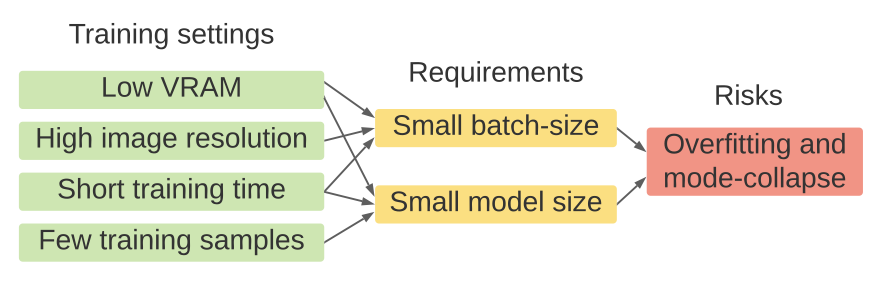
\includegraphics[width=0.5\textwidth]{Images/problems.png}
		\caption{FastGAN training challenges.} 
	\end{figure}
	In some situations a possible way to avoid these problems was the transfer-learning using pre-trained models,
	but this solution had the disadvantage of the lack of guarantee to find dataset compatible with the pre-training. 
	Another way was fine-tuning, but this gave even worse results in terms of performance.
	Those approaches were not "considered" by people who wanted to train their model from scratch, in order to 
	avoid biases typic of the fine-tuned pre-trained models; in other cases there were the necessity to train models
	with datasets containing less than 100 images.
	A possible workaround for the situation of a small dataset was dynamic data-augmentation, but the cost of SOTA models
	remained very high.\\\\
	This paper aims to learn an unconditional GAN requiring, at the same time, low computational power and small datasets
	for training. In order to do this, FastGAN has a "fast-learning" generator $G$ and a discriminator $D$ able to continuously
	return signals very useful to train G. FastGAN reaches the above objectives based on the following two techniques:
	\begin{itemize}
		\setlength\itemsep{0.01em}
		\item \textbf{Skip-Layer channel-wise Excitation module}: revises channel responses on high-scale feature-maps using
			  low-scale activations and allows to reach a faster training using a more robust gradient flow throughout the 
			  model weights;
		\item \textbf{Self-supervised discriminator $D$ trained as a feature-encoder with an extra decoder}: this discriminator
			  is forced to learn a feature-map that covers more regions from an image in input; in this way it gives richer
			  signals in order to train $G$. It has been shown that auto-encoding is the best self-supervision strategy for $D$.
	\end{itemize} 

% METHOD -------------------------------------------------------------------------

\section{Method}
\large	

\begin{figure}[H]
	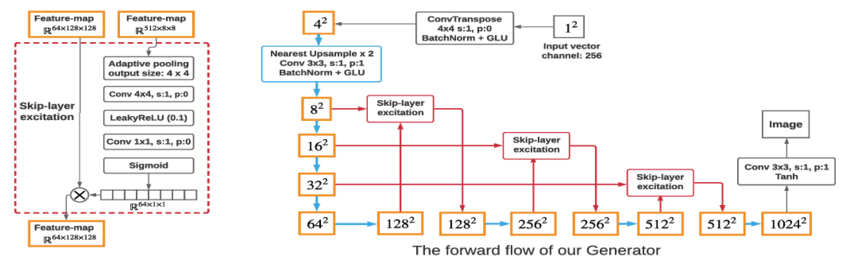
\includegraphics[width=1\textwidth]{Images/structure.png}
	\caption{
		On the left is represented the structure of the skip-layer excitation,
		on the right is represented the structure of the generator $G$. 
		Feature-maps are the yellow boxes, up-sampling structures are represented 
		by blue boxes and blue arrows, SLE modules are the red boxes.
		}
\end{figure}
In order to optimize GANs with respect to the SOTA models, in FastGAN is adopted a lightweight model, 
using a single convolutional layer on each resolution in the generator $G$; moreover, on the high resolutions
in both generator $G$ and discriminator $D$, only three channels for the convolutional layers are applied in 
input and output. As said before this structure helps making FastGAN faster to train, remaining, at the same time,
strong on small datasets. 

\subsection{Skip-Layer Channel-Wise Excitation}

In the traditional GANs the generator $G$ required more convolutional layers (and so a deeper model) to synthesize 
high resolution images, and this led to longer training times. 
In order to train such a deep model it was used the Residual structure (ResBlock) increasing the computational cost.
Traditionally ResBlock implements the skip-connection as an element-wise addition between the activations from different
convolutional layers, but with the requirement that the spatial dimensions of the activations are the same.
Moreover, previously, skip-connections were only used within the same resolution.\\\\
FastGAN, instead, uses a different approach through the two following strategies:
\begin{itemize}
	\setlength\itemsep{0.01em}
	\item {	
	In order to eliminate the complex computation of convolution, is used multiplication between activations, instead of 
	addition, giving to one side of activations the spatial dimension of $1^2$.
	}
	\item {
	Instead of performing skip-connection only within the same resolution, here is performed between resolutions with a much
	longer range ($8^2$ and $128^2$, $16^2$ and $256^2$, $32^2$ and $512^2$); this follows from the fact that an equal spatial-dimension
	is no longer required.
	}
\end{itemize} 
Using the above techniques, SLE keeps the advantages of ResBlock with a shortcut gradient flow, while not requiring an extra computation
load.

\subsection{Self-Supervised Discriminator}

% CAPITOLO 2 -------------------------------------------------------------------------	

\section{NOME}
\large


% CAPITOLO 3 -------------------------------------------------------------------------

\section{NOME}
\large


% CAPITOLO 4 -------------------------------------------------------------------------

\section{NOME}
\large


% CAPITOLO 5 -------------------------------------------------------------------------

\section{NOME}
\large


% CAPITOLO 6 -------------------------------------------------------------------------

\section{NOME}
\large


% CAPITOLO 7 -------------------------------------------------------------------------

\section{NOME}
\large


% CAPITOLO 8 -------------------------------------------------------------------------

\section{NOME}
\large


\end{document}

% COSE UTILI --------------------------------------------------------------------------

%\section*{NOME}
%\subsection*{1.1}
%\setlength{\intextsep}{0pt} --> elimina lo spazio
%\vspace{-3mm}
%\hspace*{0cm}

% Font -------------------------------------

%GRASSETTO: \textbf

% Simboli ---------------------------------

%$\leftarrow$

% Elenco puntato ----------------------

%\begin{itemize}
%\setlength\itemsep{0.01em}
%\item 1
%\item 2
%\end{itemize}

% Graffa grande -----------------------

%\[  
%    \left\{ 
%    \begin{array}{ll} 
%      \mbox{1}
%      \mbox{2}
%    \end{array}
%    \mbox{riga al lato}
%   \right. 
%\]

% Multicolonne --------------------------

% \begin{multicols}{2}
% \columnbreak
% \end{multicols}

% Algoritmi -------------------------------

%\renewcommand{\thealgorithm}{1.\arabic{algorithm}}
%\setcounter{algorithm}{0}
%\begin{algorithm}
%\footnotesize
%\caption{Nome}
%\textbf{Input:} \\
%\textbf{Output:} 

%\begin{algorithmic}[1]
%\STATE 
%\FOR{ = 0 \TO i = n} ---- \ENDFOR
%\IF{} ---- \ELSIF{} ---- \ENDIF
%\RETURN 
%\end{algorithmic}
%\end{algorithm}

% Minipage ------------------------------

%\begin{minipage}[t]{0.5\textwidth}

% queste 3 righe vanno attaccate
%\end{minipage}
%\hspace{0.02\linewidth}
%\begin{minipage}[t]{0.47\textwidth} 

%\begin{minipage}[t]{0.3\textwidth} 
%\end{minipage}

% Proof --------------------------------
%\begin{proof}[\textbf{per cambiare nome}]
%\end{proof}

